\subsubsection{Admin UI}

Das Admin UI bietet Praxisverantwortlichen die Möglichkeit die Konfiguration des Praxisrufsystems zu verwalten.
Da nur Praxisverantworliche das Admin UI verwenden dürfen, ist die Benutzeroberfläche durch ein Login geschützt.
Die entsprechenden Anmeldeinformationen müssen bei Installation des Cloud Services vom Betreiber manuell konfiguriert werden.\footnote{Siehe Anhang D}

\begin{figure}[h]
    \centering
    \begin{minipage}[b]{0.4\textwidth}
        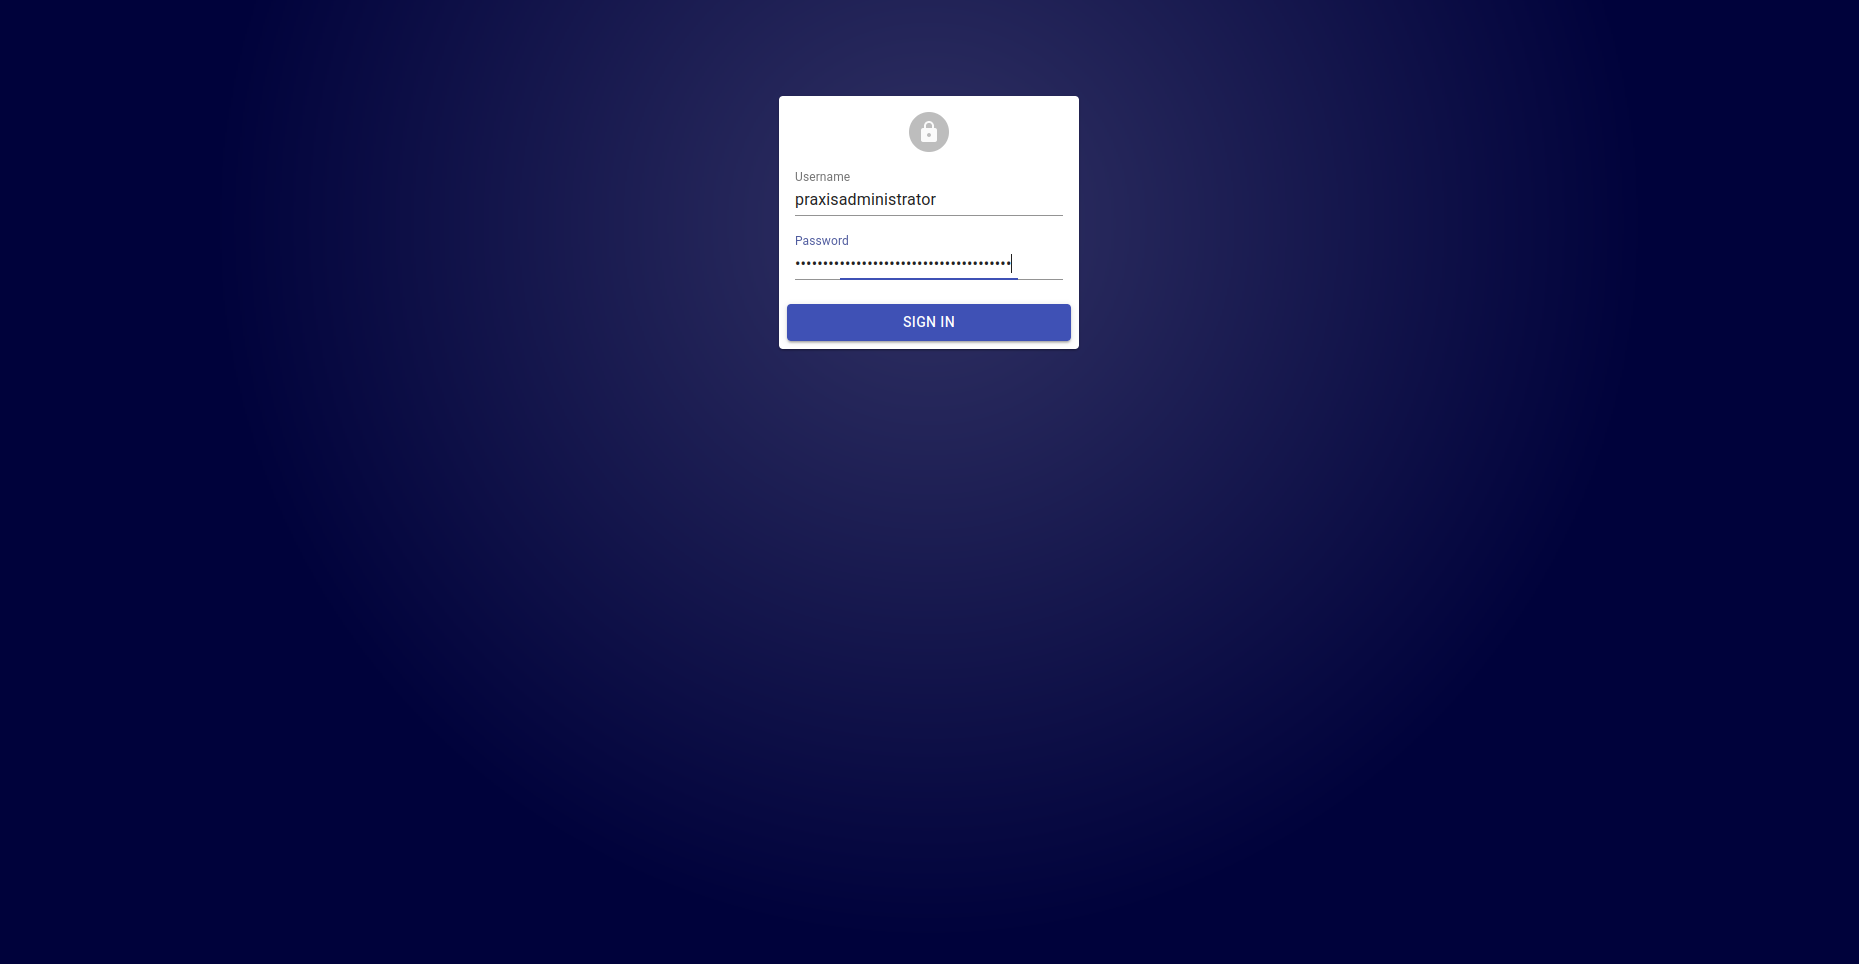
\includegraphics[width=\textwidth]{graphics/screenshots/adminui/login}
        \caption{Login}
    \end{minipage}
    \hfill
    \begin{minipage}[b]{0.4\textwidth}
        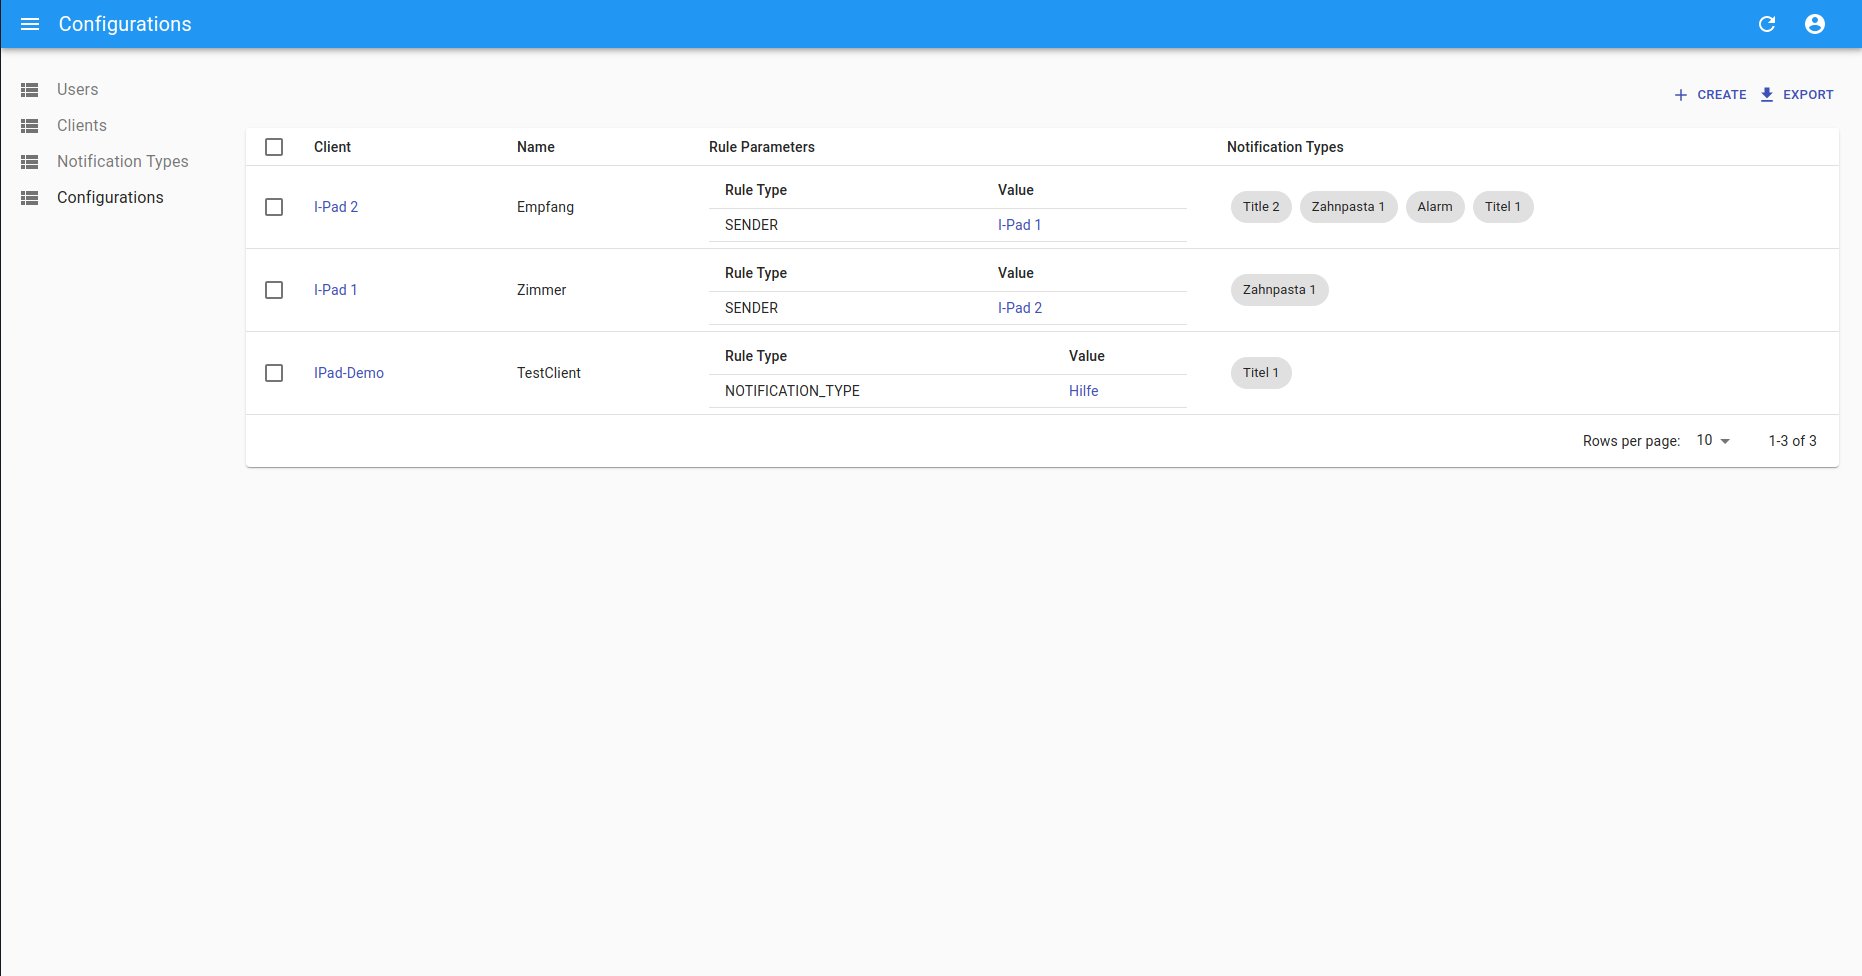
\includegraphics[width=\textwidth]{graphics/screenshots/adminui/configuration-all}
        \caption{Configuration Overview}
    \end{minipage}
    \label{fig:AdminUI-Screens1}
\end{figure}

Das Admin UI beinhaltet vier Bereiche.
Der Bereich Users dient dazu Benutzer zu erstellen, welche sich als Benutzer am Mobile Client anmelden können.
Unter dem Bereich Clients können Geräte verwaltet werden.
Jeder Client ist eindeutig einem Benutzer zugewiesen.
Im Bereich Notification Types können Benachrichtigungen verwaltet werden.
Hier wird konfiguriert, welchen Text der Button für diese Benachrichtigungen im Mobile Client hat und welchen Inhalt die Benachrichtigung hat, wenn sie versendet wird.
Unter dem Bereich Configurations wird die zentrale Konfiguration eines Clients verwaltet.
Jede Konfiguration wird genau einem Client zugewiesen.
Die Konfiguration beinhaltet eine Liste von Notification Types, welche auf dem zugewiesenen Mobile Client als Versenden Button angezeigt werden.
Weiter definiert die Konfiguration eine Liste von Regel Parametern, welche bestimmen, welche Benachrichtigungen dem zugewiesenen Client weitergeleitet werden.

\begin{figure}[h]
    \centering
    \begin{minipage}[b]{0.4\textwidth}
        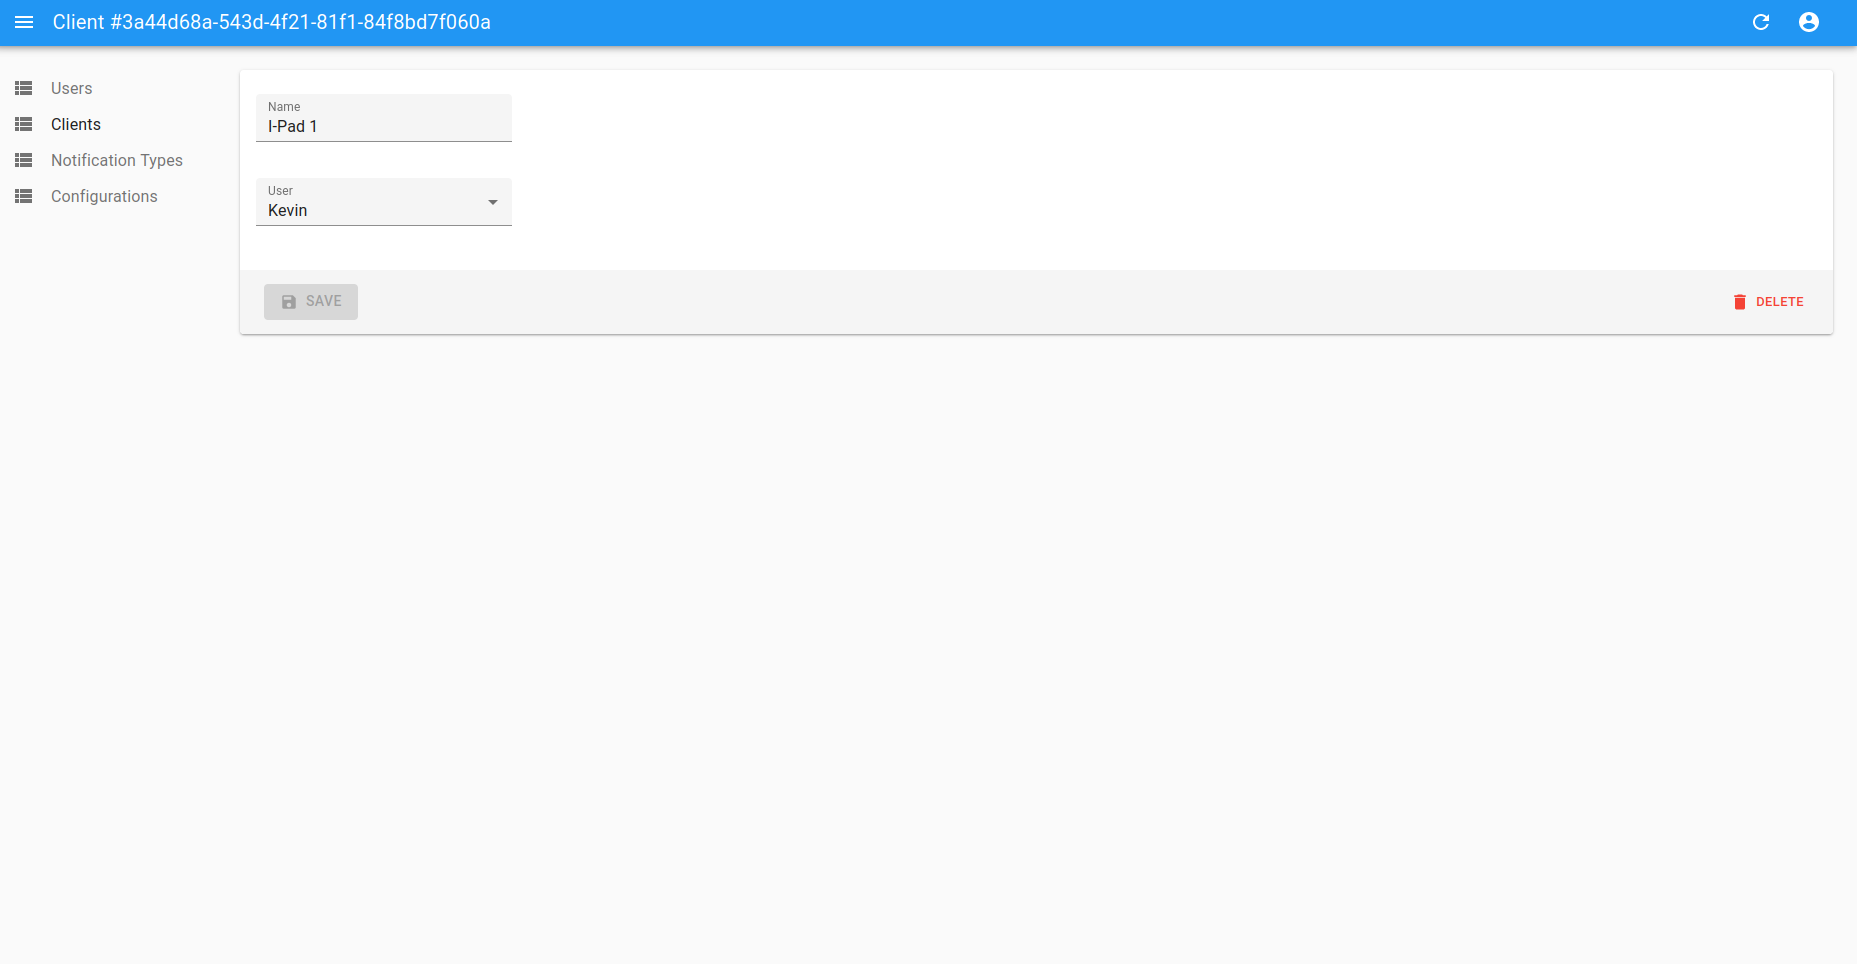
\includegraphics[width=\textwidth]{graphics/screenshots/adminui/configuration}
        \caption{Login}
    \end{minipage}
    \hfill
    \begin{minipage}[b]{0.4\textwidth}
        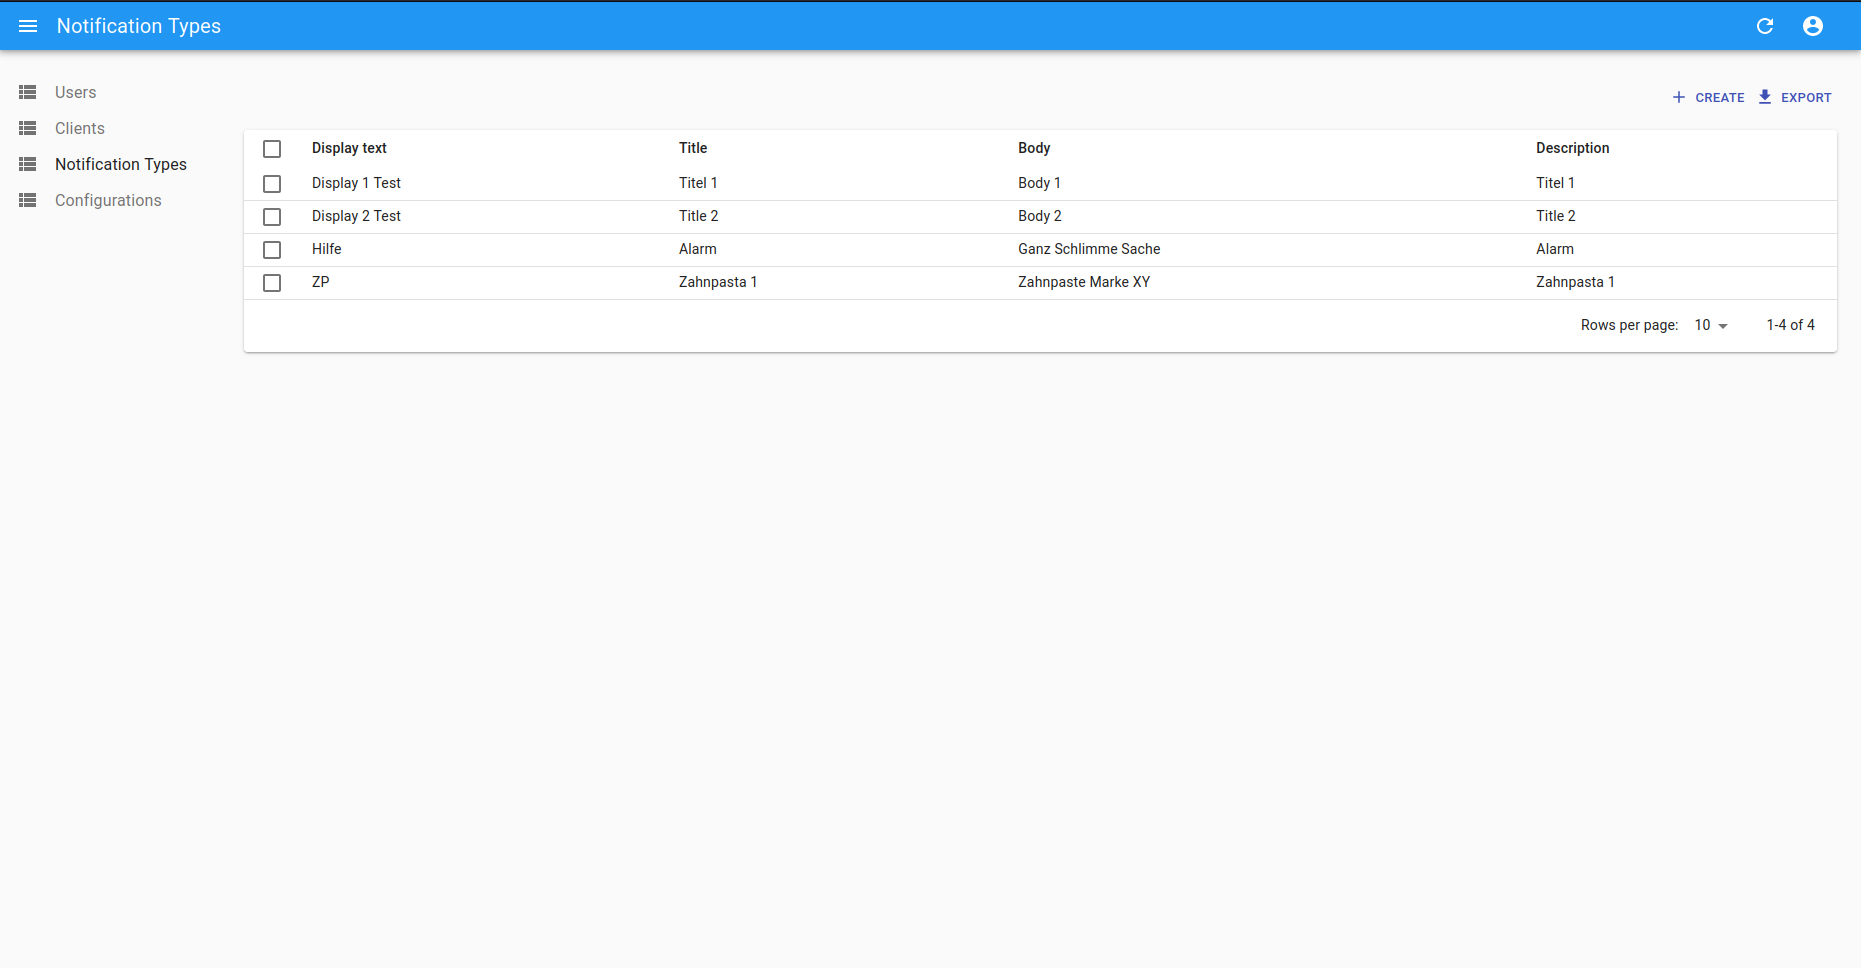
\includegraphics[width=\textwidth]{graphics/screenshots/adminui/notification-type}
        \caption{Configuration Overview}
    \end{minipage}
    \label{fig:AdminUI-Screens2}
\end{figure}

Jeder der Bereiche im Admin UI bietet dem Benutzer die Möglichkeit, den jeweiligen Teil der Konfiguration zu lesen, erstellen, bearbeiten und löschen.
Auf der Startseite jedes Bereiches wird eine Liste mit allen relevanten Einträgen angezeigt.
Mehr Informationen zur Bedienung des Admin UIs befinden sich im Benutzerhandbuch.\footnote{Siehe Anhang C}

\clearpage
